\documentclass[
	a4paper,
	12pt,
	brazilian
]{article}

\usepackage[utf8]{inputenc}
\usepackage[T1]{fontenc}

\usepackage{amsmath, amsfonts, amssymb}
\usepackage{siunitx}

\usepackage[
top=2cm,
right=3cm,
bottom=2cm,
left=3cm
]{geometry}

\usepackage{xcolor}
\usepackage{tikz}
\usepackage{import}
\usepackage{float}

\usepackage{graphicx}
\usepackage{hyperref}
\usepackage{cleveref}
\usepackage{bm}
\usepackage{multirow}
\usepackage[version=4]{mhchem}

\usepackage{config}

\begin{document}
	\section{Primeira questão}
	Calcular a pressão relativa no ponto indicado da tubulação. Resposta em \SI{}{\pascal} com uma casa decimal.\\
	\textbf{Dados:}
	\begin{itemize}
		\item Massa específica do fluido 1 = $\SI{13.1}{\gram/\centi\meter^{3}}$
		\item Massa específica do fluido 2 = $\SI{8.3}{\gram/\centi\meter^{3}}$
		\item Massa específica da água = $\SI{1000}{\kilogram/\meter^{3}}$
		\item $X=\SI{18.4}{\centi\meter}$
		\item $Y=\SI{8.3}{\centi\meter}$
		\item $Z=\SI{21.9}{\centi\meter}$
		\item $\beta=\SI{67.4}{\SIUnitSymbolDegree}$
	\end{itemize}
	\vspace{-7cm}
	\begin{flushright}
			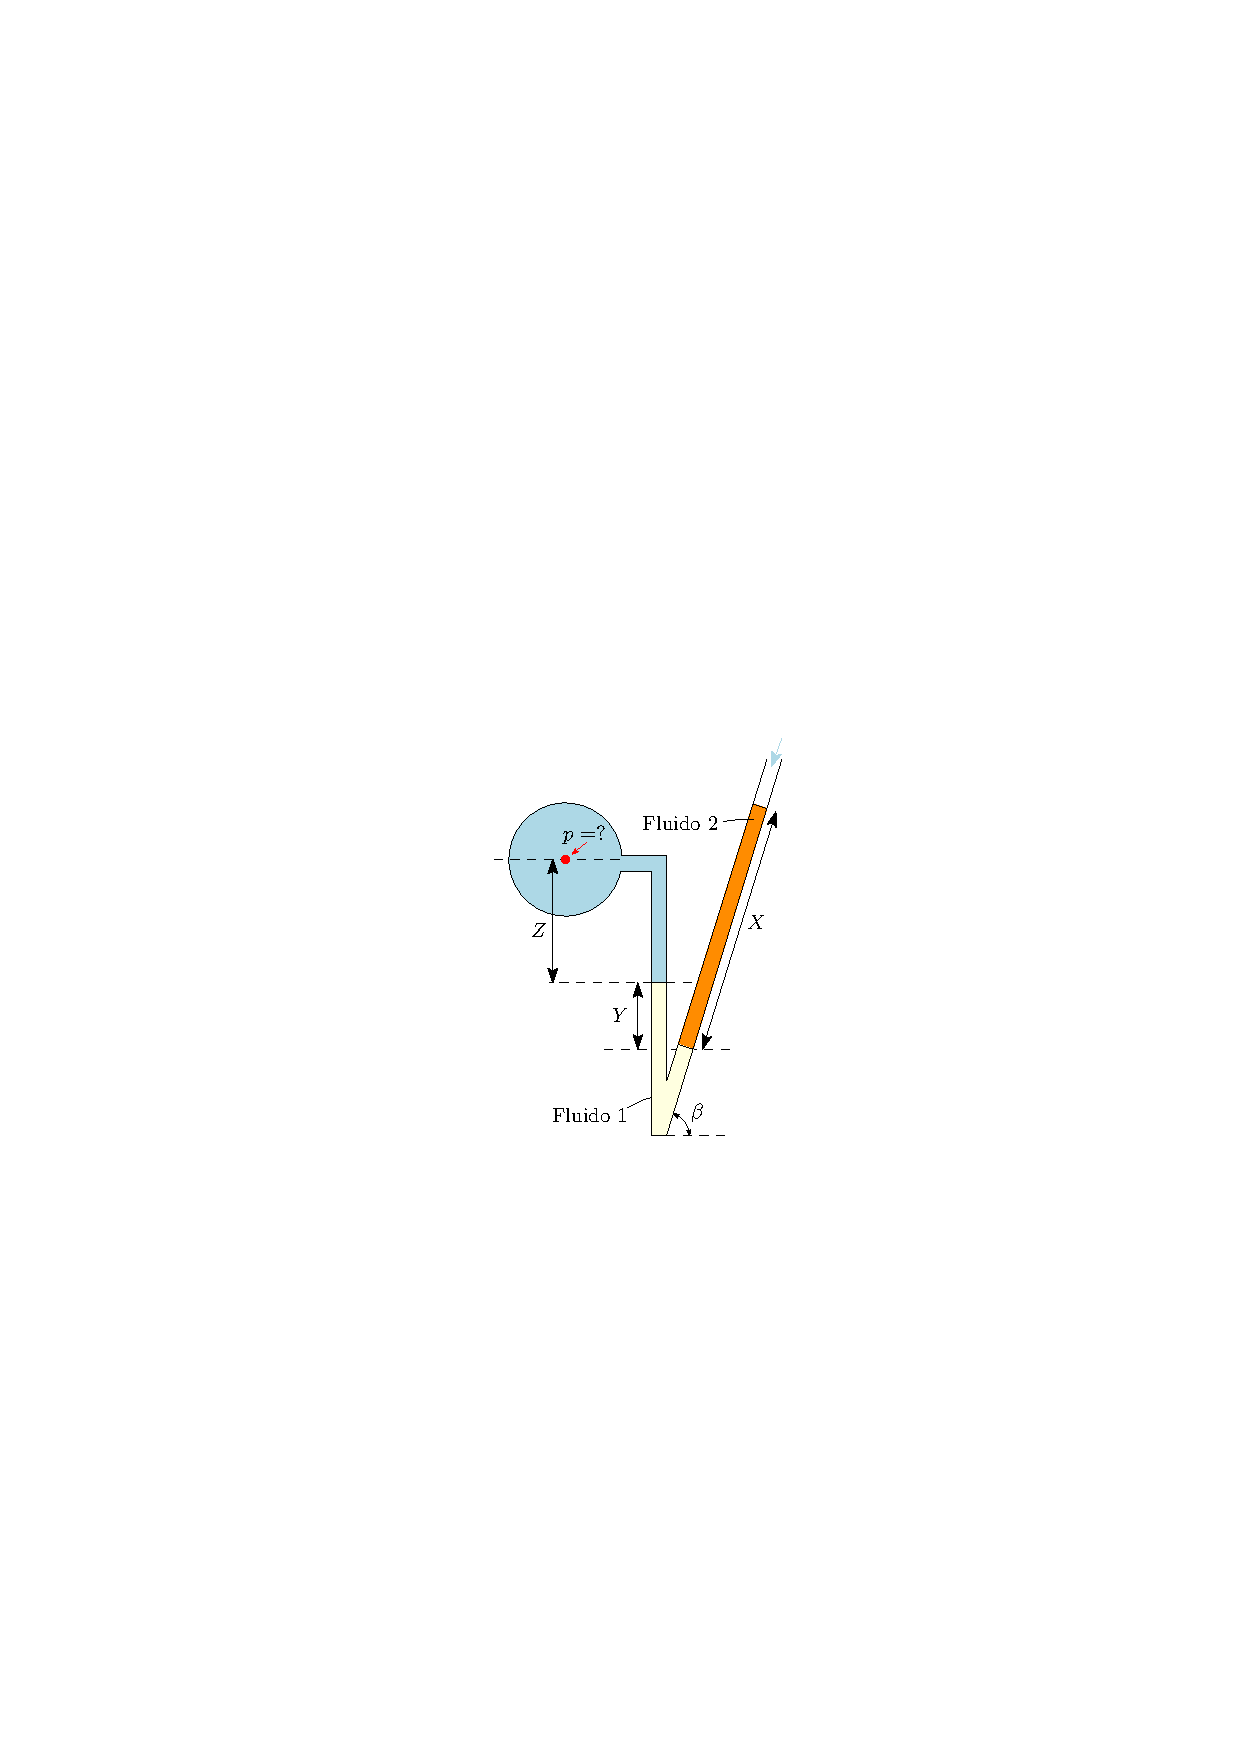
\includegraphics[width=0.4\linewidth]{assets/images/ex1}
	\end{flushright}
	\subsection{Solução}
	\begin{enumerate}
		\item[(1)] Estabelecer um referencial. É comum adotar a interface líquido-líquido.
		\begin{center}
			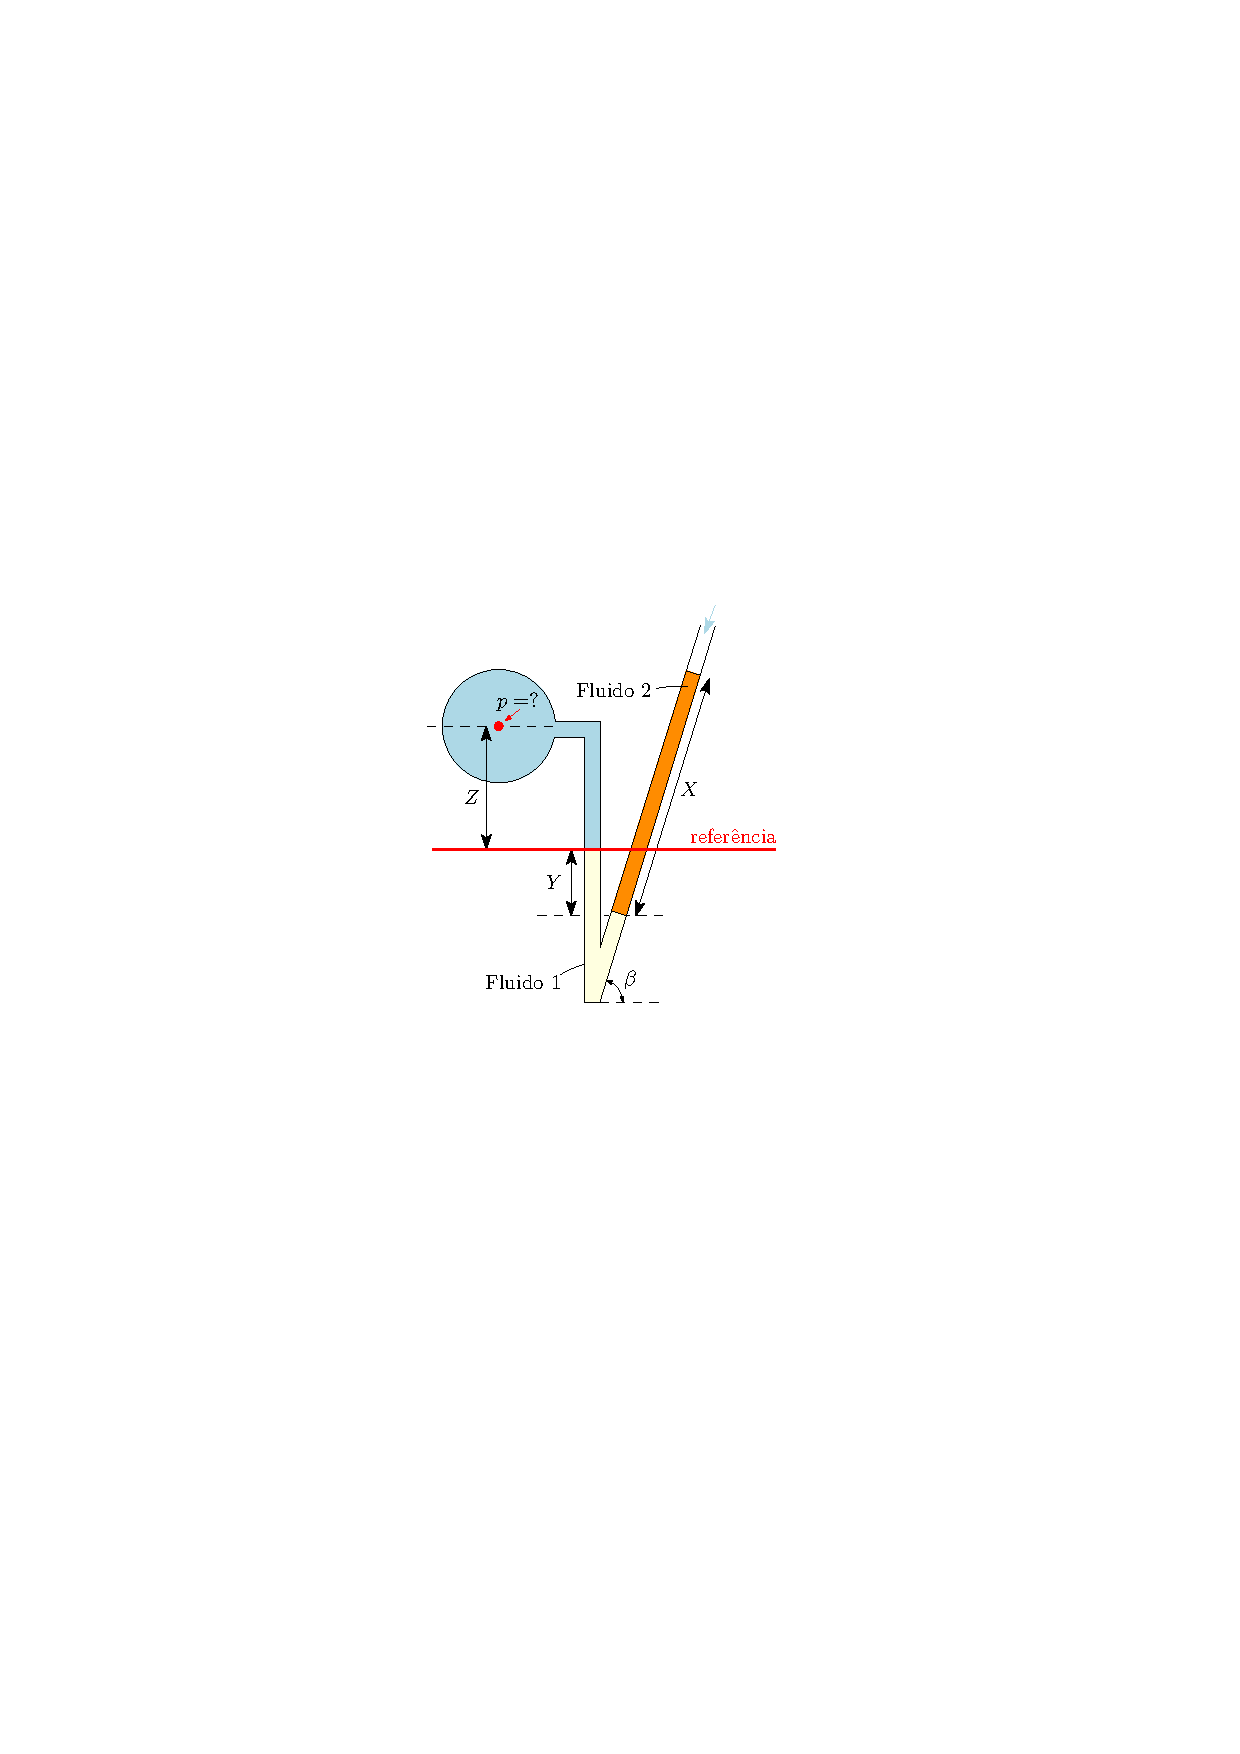
\includegraphics[width=.5\linewidth]{assets/images/referencia}
		\end{center}
		\item[(2)] Após estabelecer a cota de referência deve-se demarcar os pontos que serão analisados quanto a variação de pressão. Nesse caso, foram definidos dois pontos pertencentes à cota (1 e 2) e um ponto na superfície superior do fluido 2 (3) já que a pressão atmosférica na região simplifica os cálculos.
		\begin{center}
			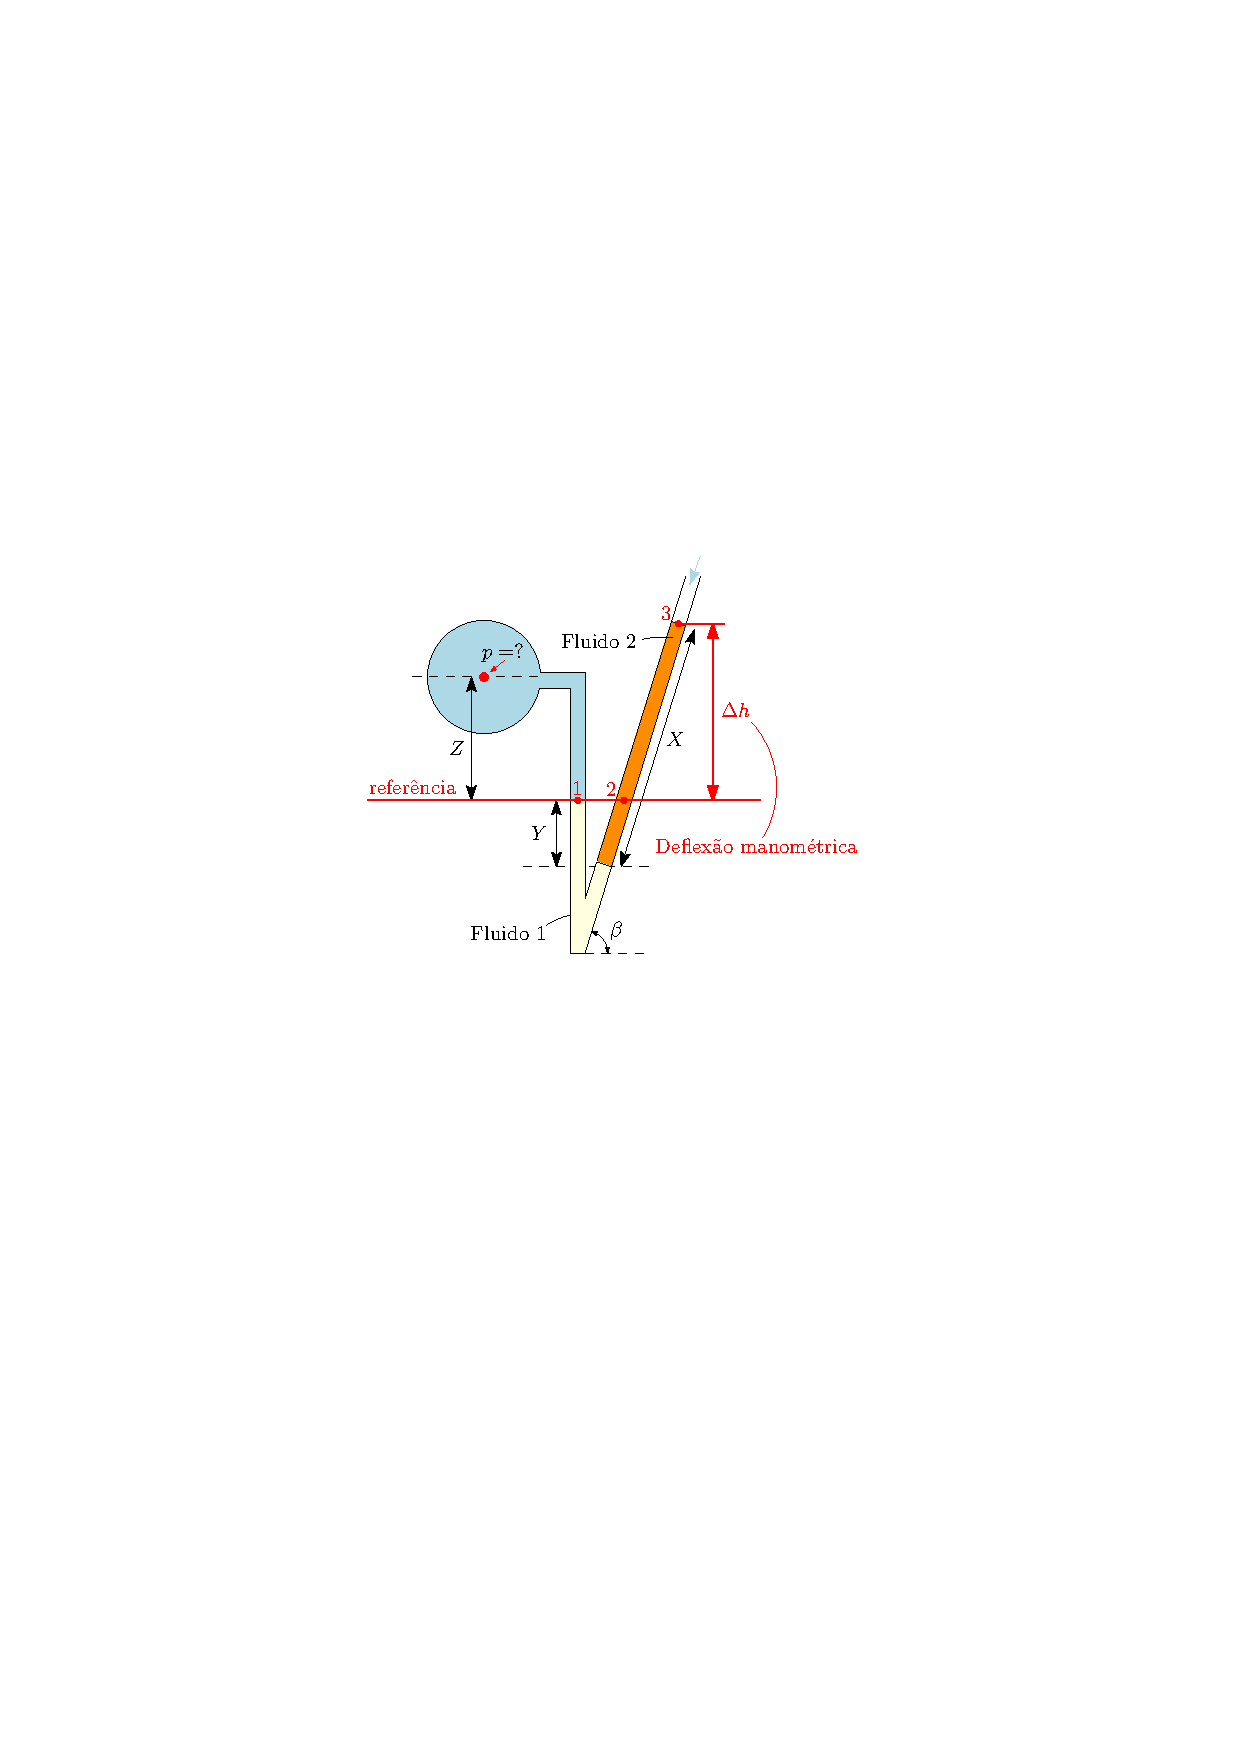
\includegraphics[width=.7\linewidth]{assets/images/pontos}
		\end{center}
		\item[(3)] Agora basta aplicação a lógica assimilada na parte do manômetros diferenciais e formular as equações para cada par de pontos como é visto abaixo
		$$
		\begin{cases}
			p_{1}-p=\gamma_{\ce{H2O}}\cdot Z\\
			p_{2}-p_{3}=\gamma_{2}\cdot\Delta h
		\end{cases}
		$$
		\item[(4)] Aplicando os conceitos vistos em hidrostática, sabemos que pontos na mesma cota apresentam a mesma pressão (1 e 2), logo
		\begin{eqnarray}
			p+\gamma_{\ce{H2O}}\cdot Z&=&p_{3}+\gamma_{2}\cdot\Delta h
		\end{eqnarray}
		\item[(5)] Como a pressão atuante em três é a atmosférica podemos desprezá-la para o sistema analisado, assim ao isolar $p$ obtemos
		\begin{eqnarray}
			p=\gamma_{2}\cdot\Delta h-\gamma_{\ce{H2O}}\cdot Z
		\end{eqnarray}
		\item[(6)] Podemos considerar, por trigonometria, que $\Delta h=X\cdot\sin\beta$ e que $\gamma=\rho\cdot g$, então
		\begin{eqnarray}
			p&=&\rho_{2}\cdot g\cdot X\cdot\sin\beta-\rho_{\ce{H2O}}\cdot g\cdot Z\\
			&=&g\cdot (\rho_{2}\cdot X\cdot\sin\beta-\rho_{\ce{H2O}}\cdot Z)
		\end{eqnarray}
		\item[(7)] Por fim, é necessário considerar o as unidades no SI e converter as massas específicas dadas em gramas por centímetro cúbico ($\SI{}{\gram/\centi\meter^{3}}$) para quilogramas por metro cúbico ($\SI{}{\kilogram/\meter^{3}}$)
		\begin{eqnarray}
			\SI{}{\dfrac{\gram}{\centi\meter^{3}}}&=&\dfrac{10^{-3}}{(10^{-2})^{3}}\SI{}{\dfrac{\kilogram}{\meter^{3}}}\\
			&=&\dfrac{10^{-3}}{10^{-6}}\SI{}{\dfrac{\kilogram}{\meter^{3}}}\\
			&=&\SI{1000}{\dfrac{\kilogram}{\meter^{3}}}
		\end{eqnarray}
		\item[(8)] Ao substituir os valores de massa específica em gramas por centímetro cúbico pelo fator (1000), obtemos que $p$ será
		\begin{eqnarray}
			p&=&8300\cdot 9.81\cdot\sin 67.4^{\circ}-1000\cdot 9.81\cdot 21.9\cdot 10^{-2}\\
			&=&\SI{73022.1}{\pascal}\approx\SI{73}{\kilo\pascal}
		\end{eqnarray}
	\end{enumerate}
\end{document}